\documentclass[11pt,twoside]{article}
\usepackage{etex}
\newcommand{\num}{6{} }

\raggedbottom

%geometry (sets margin) and other useful packages
\usepackage{geometry}
\geometry{top=.8in, left=.8in,right=.8in,bottom=.8in}
 \usepackage{graphicx,booktabs,calc}

%=== GRAPHICS PATH ===========
%\graphicspath{{./140408-Images/}}
% Marginpar width
%Marginpar width
\newcommand{\pts}[1]{\marginpar{ \small\hspace{0pt} \textit{[#1]} } }
\setlength{\marginparwidth}{.5in}
%\reversemarginpar
%\setlength{\marginparsep}{.02in}

%% Fonts
% \usepackage{fourier}
% \usepackage[T1]{pbsi}

\usepackage{lmodern}
\usepackage[T1]{fontenc}
%\usepackage{minted}

\usepackage{rotating, soul}
%% Cite Title
\usepackage[style=authoryear,backend=biber,natbib,maxcitenames=2,doi=false,isbn=false,url=false,eprint=false,uniquename=false]{biblatex}
\addbibresource{../../References/odx-model2.bib}
 
%%for tables
\usepackage{multirow} % Required for multirows
\usepackage{booktabs}
\usepackage{longtable}
\usepackage{rotating}

%%% Counters
\usepackage{chngcntr,mathtools}
\counterwithout{figure}{section}
\counterwithout{table}{section}

\numberwithin{equation}{section}

%% Captions
\usepackage{caption}
\captionsetup{
  labelsep=quad,
  justification=raggedright,
  labelfont=sc
}

%AMS-TeX packages
\usepackage{amssymb,amsmath,amsthm}
\usepackage{bm}
\usepackage[mathscr]{eucal}
\usepackage{colortbl}
\usepackage{color}


\usepackage{epstopdf,subfigure,hyperref,enumerate,polynom,polynomial}
\usepackage{multirow,minitoc,fancybox,array,multicol}

\definecolor{slblue}{rgb}{0,.3,.62}
\hypersetup{
    colorlinks,%
    citecolor=blue,%
    filecolor=blue,%
    linkcolor=blue,
    urlcolor=slblue
}

%%%TIKZ
\usepackage{tikz}

\usepackage{pgfplots}
\usepackage{pgfplotstable}
\usepackage{pgfgantt}
\pgfplotsset{compat=newest}

\usetikzlibrary{shapes.geometric, arrows}
\usetikzlibrary{arrows,shapes,positioning}
\usetikzlibrary{decorations.markings}
\usetikzlibrary{shadows,automata}
\usetikzlibrary{patterns}

\tikzstyle{startstop} = [rectangle, rounded corners, minimum width=3cm, minimum height=1cm,text centered, text width=3cm, draw=black, fill=white!30]
\tikzstyle{io} = [trapezium, trapezium left angle=70, trapezium right angle=110, minimum width=1cm, minimum height=1cm, text centered, text width=2cm, draw=black, fill=white!30]
\tikzstyle{process} = [rectangle, minimum width=3cm, minimum height=1cm, text centered, text width=3cm, draw=black, fill=white!30]
\tikzstyle{decision} = [diamond, minimum width=3cm, minimum height=1cm, text centered, text width=3cm, draw=black, fill=white!30]
\tikzstyle{arrow} = [thick,->,>=stealth]

%\usetikzlibrary{circuits.ee.IEC}
\usetikzlibrary{decorations.text}
% For Sagnac Picture
\usetikzlibrary{%
    decorations.pathreplacing,%
    decorations.pathmorphing%
}

%
%Redefining sections as problems
%
\makeatletter
\newenvironment{question}{\@startsection
	{section}
	{1}
	{-.2em}
	{-3.5ex plus -1ex minus -.2ex}
    	{1.3ex plus .2ex}
    	{\pagebreak[3]%forces pagebreak when space is small; use \eject for better results
	\large\bf\noindent{Question }
	}
	}
	%{\vspace{1ex}\begin{center} \rule{0.3\linewidth}{.3pt}\end{center}}
	%\begin{center}\large\bf \ldots\ldots\ldots\end{center}}
\makeatother

%
%Fancy-header package to modify header/page numbering
%
%\renewcommand{\chaptermark}[1]{ \markboth{#1}{} }
\renewcommand{\sectionmark}[1]{ \markright{#1}{} }

\usepackage{fancyhdr}
%\pagestyle{fancy}
%\addtolength{\headwidth}{\marginparsep} %these change header-rule width
%\addtolength{\headwidth}{\marginparwidth}
%\fancyheadoffset{30pt}
%\fancyfootoffset{30pt}
%\fancyhead[LO,RE]{\small  \it \nouppercase{\leftmark}}
%\fancyhead[RO,LE]{\small Page \thepage}
%\fancyfoot[RO,LE]{\small }% PR \num S-2015}
%\fancyfoot[LO,RE]{\small }%\scshape MODL}
%\cfoot{}
\renewcommand{\headrulewidth}{0.1pt}
\renewcommand{\footrulewidth}{0pt}
%\setlength\voffset{-0.25in}
%\setlength\textheight{648pt}


\usepackage{paralist}


%%% FORMAT PYTHON CODE
\usepackage{listings}
% Default fixed font does not support bold face
\DeclareFixedFont{\ttb}{T1}{txtt}{bx}{n}{8} % for bold
\DeclareFixedFont{\ttm}{T1}{txtt}{m}{n}{8}  % for normal

% Custom colors
\usepackage{color}
\definecolor{deepblue}{rgb}{0,0,0.5}
\definecolor{deepred}{rgb}{0.6,0,0}
\definecolor{deepgreen}{rgb}{0,0.5,0}

%\usepackage{listings}

% % Python style for highlighting
% \newcommand\pythonstyle{\lstset{
% language=Python,
% basicstyle=\footnotesize\ttm,
% otherkeywords={self},             % Add keywords here
% keywordstyle=\footnotesize\ttb\color{deepblue},
% emph={MyClass,__init__},          % Custom highlighting
% emphstyle=\footnotesize\ttb\color{deepred},    % Custom highlighting style
% stringstyle=\color{deepgreen},
% frame=tb,                         % Any extra options here
% showstringspaces=false            %
% }}

% % Python environment
% \lstnewenvironment{python}[1][]
% {
% \pythonstyle
% \lstset{#1}
% }
% {}

% % Python for external files
% \newcommand\pythonexternal[2][]{{
% \pythonstyle
% \lstinputlisting[#1]{#2}}}

% % Python for inline
% \newcommand\pythoninline[1]{{\pythonstyle\lstinline!#1!}}


\newcommand{\osn}{\oldstylenums}
\newcommand{\dg}{^{\circ}}
\newcommand{\lt}{\left}
\newcommand{\rt}{\right}
\newcommand{\pt}{\phantom}
\newcommand{\tf}{\therefore}
\newcommand{\?}{\stackrel{?}{=}}
\newcommand{\fr}{\frac}
\newcommand{\dfr}{\dfrac}
%\newcommand{\ul}{\underline}
\newcommand{\tn}{\tabularnewline}
\newcommand{\nl}{\newline}
\newcommand\relph[1]{\mathrel{\phantom{#1}}}
\newcommand{\cm}{\checkmark}
\newcommand{\ol}{\overline}
\newcommand{\rd}{\color{red}}
\newcommand{\bl}{\color{blue}}
\newcommand{\pl}{\color{purple}}
\newcommand{\og}{\color{orange!90!black}}
\newcommand{\gr}{\color{green!40!black}}
\newcommand{\nin}{\noindent}
\newcommand{\la}{\lambda}
\renewcommand{\th}{\theta}
\newcommand{\al}{\alpha}
\newcommand{\G}{\Gamma}
\newcommand*\circled[1]{\tikz[baseline=(char.base)]{
            \node[shape=circle,draw,thick,inner sep=1pt] (char) {\small #1};}}

\newcommand{\bc}{\begin{compactenum}[\quad--]}
\newcommand{\ec}{\end{compactenum}}

\newcommand{\p}{\partial}
\newcommand{\pd}[2]{\frac{\partial{#1}}{\partial{#2}}}
\newcommand{\dpd}[2]{\dfrac{\partial{#1}}{\partial{#2}}}
\newcommand{\pdd}[2]{\frac{\partial^2{#1}}{\partial{#2}^2}}


%%%%%%%%%%%%%%%%%%%%%%%%%%%%%%%%%%%%%%%%%%%%%%%%%%%
%%%%%%%%%%%%%%%%%%%%%%%%%%%%%%%%%%%%%%%%%%%%%%%%%%%

\begin{document}
\title{Review of origin-destination estimation methods for public transit systems}
\author{}
\date{\small\today}
\maketitle

%\thispagestyle{empty}

%\tableofcontents


\section{A brief background to travel demand modeling}



%\item Brief history of origin-destination modeling

Estimating travel demand is a key input to service planning. An origin-destination model that predicts the decisions made by riders based on good assumptions is essential for designing an efficient transit system. However, a huge amount of Data is needed to achieve this. In the past, the only methods of collecting this data were direct methods such as home surveys and road surveys (direct sampling estimation) \citep{vitiStateofartODMatrix2008, netoStatisticalModelsEstimation2017}. These methods are useful in describing some characteristics of the respondents that are otherwise not collected such as age, gender, income, occupation, and detailed travel information like trip purpose and mode choice \citep{zannatEmergingBigData2019}. However, such methods are not without flaws. The data needed is collected at big intervals, maybe once or twice in a decade, because an enormous sample data is needed which is expensive \citep{netoStatisticalModelsEstimation2017}. the process is also subject to biases and may take a very long time for the data to be collected, analyzed, and finally be used to develop a model.

Early classical modeling included two major approaches, the most commonly used are the Four Stage (step) Model (FSM), and the Activity Based Model \citep{rasouliCriticalReviewCurrent2017, shanComparisonTripGeneration2012}. FSM was first employed in the 1950s and was developed for large scale infrastructure projects. Each of its four stages (Trip generation, trip distribution, modal split, and trip assignment) can be carried out using many different models which range from simple to very sophisticated and comprehensive. 

the first step of FSM is known as Trip Generation. It is a zone-wise analysis to give an idea of how many trips are generated and attracted from and to different zones in the study area. It uses methods like the Growth factor model and Regression model. In the second step, the trip distribution, Casey introduced the Gravity Model, which employs the physics-based law of gravitational attraction to spatially assign trips in a network \citep{willumsenEstimationODMatrix1978, ekowicaksonoEstimatingOriginDestinationMatrix2016}. Many researchers such as \citet{hogbergEstimationParametersModels1976, robillardEstimatingODMatrix1975, lowNEWAPPROACHTRANSPORTATION1972} used different types of the gravity model for their research \citep{willumsenEstimationODMatrix1978}.  In the third step of FSM, the modal split, models including the binary logit model and the multinomial logit model are used to determine the choice of passengers and split the trips mode-wise . Then in the Traffic Assignment, which is the final step, assignment models such as the all-or-nothing, user-equilibrium, and system-optimum are commonly utilized to distribute trips within the network \citep{TripAssignment}.

In the 1970s, researchers took advantage of big data generated from traffic monitoring systems to develop indirect mathematical models such as the ones based on maximum entropy and minimum information principles developed by \citet{vanzuylenMostLikelyTrip1980} and \citet{willumsenEstimationODMatrix1978} to obtain OD matrices.  

FSM dominated the history of demand forecasting and measuring the performance of transit systems \citep{mcnallyFourStepModel2000}. However, while FSM and other trip-based models are effective for estimating the impact of the transportation infrastructure development and expansion, they do not provide a valid representation of the underlying travel behavior (they can tell what people do but not why they do it) \citep{mcnallyActivityBasedApproach2007}. They are, therefore, unable to be responsive to the changing policies oriented towards management rather than expansion. This means that they cannot tell us how people might react to new approaches or travel alternatives. As a result of these weaknesses, the development of alternative approaches was stimulated. The study of \citet{mitchellUrbanTrafficFunction1954} has established the link of travel and activities and called for a comprehensive framework for travel behavior. And in the 1970s, the study of the activity based approach was first analyzed in depth. The motivation behind this approach was that the reflection of the link between travel and activities and understanding of activity behavior is fundamental, and understanding travel behavior comes second \citep{mcnallyActivityBasedApproach2007}.


%\begin{itemize}
%\item Answering the key questions: who, what, when, where?
%  \begin{itemize}
%  \item Who are the key contributors to this field
%  \item what exactly has been done? Which modeling approaches have been employed?
 % \item Where have they been deployed? What has been the impact?
%  \item When were these efforts made? (chronological aspect)
%  \end{itemize}
%\end{itemize}








\section{Origin Destination Transfer Inference}
% a transitional paragraph motivating the need for ODX is needed here. why we need ODX models, what are the benefits, and what are the new opportunities given the era of big data and ML?
%\subsection {The Need for ODX}

Origin, destination, and interchange inference (ODX) method is a recent research outcome that utilizes automatic data collection systems which provide a very rich new data source that is both realistic and up to date. 

Analyzing a transit network using ODX provides a more accurate analysis of the network usage and a level of detailed geographical disaggregate data on passengers trips that was unavailable with previous data collection methods. This offers a complete and reliable picture of riders’ activity and route choices that does not rely on assumptions as is the case with older models.

It can also provide planners with specific information about where to target their available resources and make adjustments to achieve maximum efficiency of the transit network and what the possible effects of those adjustments are \citep{vanderwaartPlanningTransitNetworks2016}. 





In recent years, various OD estimation methods using the trip-chaining approach have attracted the attention of researchers. And a new method of inferring the origin destination matrix using automated data collection systems (ADCS) called origin destination transfer (interchange) inference coined by Gordon as (ODX) was  developed \citep{vanderwaartPlanningTransitNetworks2016, sanchez-martinezInferencePublicTransportation2017}. The process  is divided into three steps: origin inference, destination inference, and transfer (i.e., interchange) which mainly aims to find out whether the inferred alighting location is the real destination for that particular trip. 
 
A number of studies used different methodologies to infer OD matrices for transit trips using smart card data such as the study by \citet{wangBusPassengerOrigindestination2010, nassirTransitStopLevelOrigin2011, gordonIntermodalPassengerFlows2012}

The validity of these estimation methods has not been extensively investigated, because passengers are often required to tap their smart cards only when boarding a public transport service (in open systems), resulting in datasets that lack data about passengers' alighting \citep{alsgerValidatingImprovingPublic2016}. However, with ADCS data which are a major improvement over the traditional data collection methods, inferring origin destination matrices is possible with minimal costs.

ODX uses key ADCS like automatic vehicle location, automatic fare collection, and automatic passenger counting instead of manual surveys to infer destinations and transfers in open systems, which is usually the case, or only to infer transfers in closed systems where each OD pair is given. Some trips cannot be inferred however due to errors, incomplete data, assumptions of the model not being fulfilled, and passengers who do not use farecards. Therefore, the OD matrix needs to be scaled up to full demand using method such as iterative proportional fitting (IPF) \citep{vanderwaartPlanningTransitNetworks2016, cuiBusPassengerOriginDestination2006}. 







\subsection{Automated Data Collection Systems (ADCS)}

The origin destination matrix is the primary input for the public transit systems modeling approaches \citep{wongEstimationOrigindestinationMatrices2005}. In the past, OD matrices were only calculated when a network level passenger survey was being conducted which were taken in very long intervals. Also, OD estimation was not the primarily purpose for conducting them \citep{ben-akivaDATAFUSIONMETHODS1989} which meant that a relatively recent single route or network matrix is typically unavailable \citep{cuiBusPassengerOriginDestination2006}. 

In recent years, there have been rapid advancement of information and communication technology which range from sources specific to public transport, like smart cards used for automatic fare collection and global positioning system (GPS) for automatic vehicle location (AVL), to more generic data like digital footprints of mobile phone users \citep{zannatEmergingBigData2019}. This resulted in systems that can continuously collect and store raw data that can explain human mobility patterns at much lower costs without needing any human intervention \citep{cuiBusPassengerOriginDestination2006}  which led the resolution of the collected data to reach the level of the individual passenger \citep{nassirTransitStopLevelOrigin2011}. These sources have the advantage of near or real time data collection with larger sample sizes that contains much more detailed and accurate individual level data which opens the possibility for more dynamic research in this field \citep{zannatEmergingBigData2019}. However, the public transit industry has yet to implement the full potential of these new sources \citep{cuiBusPassengerOriginDestination2006}. 

%if both automatically and manually collected data are available, then the OD matrix estimation models generated from ADCS data can be validated and calibrated using survey data \citep{cuiBusPassengerOriginDestination2006}

The main automated data collection systems are Automatic Vehicle Location,  Automatic Passenger Count system, and  Automatic Passenger Count system. Since these sources cover different parts of transit. They can give a much more reliable and accurate information if they are used together. However, it isn't a straight forward process. these systems are not usually designed to be used together and provide integrated data or for generating an OD matrix at all. Hence, additional processing of data is required to make it useful \citep{zhaoPlanningAnalysisImplications2004} and up to date OD matrices can be expected to be available much more frequently as a result due to the reduced costs, larger sample sizes, and suitability for automation \citep{cuiBusPassengerOriginDestination2006}. 




\begin{itemize}
\item Automatic Fare Collection system AFC

The automated fare collection system has been increasingly popular in transit systems around the world \citep{huangMethodBusOD2020}. Many Cities have their own Smart fare card system such as London (Oyster card), New York (Smart Link), Boston (Charlie card), Beijing (Yika tong), and Hong Kong (Octopus card) \citep{zannatEmergingBigData2019}. Passengers are required to tap their cards during entry and/or exit depending on the specific transit agency's arrangement. This information is collected by the AFC system and can be used for OD inference \citep{cuiBusPassengerOriginDestination2006}.

%at both boarding and alighting times, which provides readily available origins and destination data, or only at boarding time which requires the destinations to be inferred
%Among different novel data sources, smart card data has the capability to enhance existing decision-making tools, minimizing the complexities associated with conventional data collection systems (e.g., of onboard surveys)42 \citep{zannatEmergingBigData2019}.

\item Automatic Vehicle Location system AVL

The location of vehicles in a network is very important for estimating OD matrices. In bus systems, AFC systems do not usually know their location and only collect payment records. GPS is typically used for AVL, sometimes supplemented by odometer readings\citep{vanderwaartPlanningTransitNetworks2016}. If It is installed in the vehicle, time and location of each payment can be collected  \citep{cuiBusPassengerOriginDestination2006}\citep{zannatEmergingBigData2019}. But if AVL data in not available, other method to infer the location of the bus are used such as using the bus schedule \citep{cuiBusPassengerOriginDestination2006}




\item Automatic Passenger Count system APC

With sensors installed on the doors of buses, the number of passengers entering and exiting at each stop is recorded. The main purpose of APC is to provide the time, location, and total number of passengers boarding and alighting and the total number of passengers on the vehicle \citep{vanderwaartPlanningTransitNetworks2016} \citep{cuiBusPassengerOriginDestination2006}. 


\end{itemize}

%Mobile phone data At present, most individuals carry mobile phone almost everywhere, which results in mobile phone data the largest human mobility data source8. There are broadly two sources of mobile phone data—cellular network-based data and smartphone sensor-based data69. Cel-lular network-based data are collected by telecommunication companies. Two types of network-based data have been used in the contemporary PT studies: call data record (CDR) and global system for mobile com-munication (GSM) data1, 43. CDR data com-prises a set of phone activity (phone call, text message or Internet access) recordsalong with the time and location informa-tion of cell towers channeling the call. The GSM data are generated from an interaction between a device and the mobile network as long as it is turned on69. For a single mobile phone, CDR or GSM data are dispersed and provide very little information. However, aggregation of thousands of mobile phone data overcomes the above-mentioned limi-tation1. Among the two types, GSM data has a higher frequency compared to CDR data, but is typically more difficult to get access to. CDR data on the other hand is routinely saved by the mobile phone companies for billing purposes and involves no additional effort in data provision.
%On the other hand, smartphone sensor-based data can be collected by dedicated applications69. For example, check in information from social media (Twitter, Facebook, etc.) or popular sports tracking apps provide higher spatial resolution data compared to network-based data. However, this form of data is associated with serious sam-pling bias and poor temporal granularity; there-fore, very few studies used this data form for PT research58. Nevertheless, advancement of Internet and smartphone technology provides a unique opportunity to transport planners/modelers to estimate demand fluctuations under special events \citep{zannatEmergingBigData2019}


\subsection{Summary of ODX relevant work}

\citet{wangBusPassengerOrigindestination2010} successfully implemented ADCS archived data to analyze the bus passengers' travel behavior. He based his work on the trip chaining principles applied in Chicago by \citet{cuiBusPassengerOriginDestination2006} to infer boardings and alightings and to analyze the interchange patterns of London's TFL bus network passengers and distinguish between linked and unlinked trips. Wang distinguished his results by being the first to validate his work using manual surveys (the Bus Passenger Origin and Destination(BODS) survey data). Similarly, \citet{nassirTransitStopLevelOrigin2011} proposed two new models to estimate the alighting stop considering passenger trip chaining relying on AFC, APC, and transit schedule data (GTFS), in the Minneapolis–Saint Paul, Minnesota, area, to estimate passenger origins and destinations at the level of individual stops. They validated their output by comparing it to APC data with vehicle location data (APC-VL). Building upon the work done by \citet{wangBusPassengerOrigindestination2010}, \citet{gordonIntermodalPassengerFlows2012} expanded the methods used by Wang to include the rail system and presented methods for inferring the full journeys of all passengers on a large public transit system which was scaled up to include the passengers who do not use farecards using a modified IPF method. His results showed that reliance on small and infrequent sample can be avoided and that the process can be implemented on a daily basis for the whole network.
 
\citet{chenBusPassengerOriginDestination2013a} inferred boarding and alighting locations in Chongqing, China, without GPS data. They were the first to attempt to create an algorithm to use stop Geographic Information System (GIS) and dual-direction bus stop group to estimate the traveling direction and boarding location. \citet{zengDevelopNewYork2015} take a unique and novel approach of inferring each passenger's full journey in the New York City called ``Dynamic Transfer Link''. It creates an ``automatic, error-tolerant, and analyst-free daily re-calibration'' of the the shortest path model.  The research showed the feasibility of automation in large scale transit planning.
 
\citet{alsgerUseSmartCard2015, alsgerValidatingImprovingPublic2016} used smart card fare data from Queensland, Australia, with the advantage of having both boarding and alighting information, to assess the validity of previously used methods of estimating OD matrices and the effects of their assumptions (allowable transfer time, walking distance, last destination). They also proposed an algorithm in 2015 and a revised algorithm in 2016 for using individual user transactions for OD matrix generation. Their findings indicated that the assumed allowable transfer time does not have a significant impact on the OD matrices and that most passengers (90 percent) are willing to walk less than 10 minutes for transfers and most of them return to their first origin.

On the other hand, \citet{vanderwaartApplicationsInferredOrigins2017} focused on the applications of ODX rather than improving the algorithm. They used an ODX data set provided by the MBTA from 2014 to propose a new service planning procedure to determine needed service changes in specific locations of interest by calculating the number of passengers who would benefit from these changes. The results of this procedure would provide planners with better information than what is available otherwise and would support decision making when allocating the scarce resources available.

More recently and unlike earlier models that disregarded the number of transfers on path choice or the effect of the time spent waiting or in vehicles, \citet{sanchez-martinezInferencePublicTransportation2017} developed a dynamic programming model based on a generalized disutility minimization objective to try to find the path that the passenger will most likely take. This model is being used to infer OD matrices in Boston, Massachusetts, and is producing better results than previously applied models.


%Revive this table later

%\begin{sidewaystable}[h!]
 % \begin{center}
 %   \caption{ODX relevant work.}
 %   \label{tab:table2}
 %   \begin{tabular}{l|l|l|l}
 %     \textbf{Article} & \textbf{Focus} & \textbf{Used data} & \textbf{Findings}\\ 

  %    \hline

% eg     \citep{nassirTransitStopLevelOrigin2011} & proposing two models to estimate alighting stops... & AFC, AVL, and transit schedule data (GTFS)& ....\\ 


%      \citep{wangBusPassengerOrigindestination2010} & infer boardings and alightings and to analyze the interchange patterns of London's TFL bus network passengers and distinguish between linked and unlinked trips & 0 & 0\\ 

%
 %     \citep{nassirTransitStopLevelOrigin2011} & 0 & 0 & 0\\ 


 %     \citep{gordonIntermodalPassengerFlows2012} & 0 & 0 & 0\\ 


 %     \citep{chenBusPassengerOriginDestination2013a}& 0 & 0 & 0\\ 


 %     \citep{zengDevelopNewYork2015}& 0 & 0 & 0\\ 


  %    \citep{alsgerValidatingImprovingPublic2016} & 0 & 0 & 0\\ 


  %    \citep{vanderwaartApplicationsInferredOrigins2017}& 0 & 0 & 0\\ 


%      \citep{sanchez-martinezInferencePublicTransportation2017} & 0 & 0 & 0\\ 



%       etc....& etc.... & etc.... & etc....\\ 


%    \end{tabular}
%  \end{center}
%\end{sidewaystable}






\subsection{General OD matrix estimation approach using ADCS}


%A general approach Provided by \citep{cuiBusPassengerOriginDestination2006} involves the following three steps:

%\begin{itemize}
%\item Process the raw ADC data to obtain a sample set of boarding and alighting counts which are usually provided by an APC system, a sample passenger trip OD matrix which will be our seed matrix and transfer flows which are generally provided by an AFC system.

%\item Combine the marginal values and the seed matrix using a statistical technique to produce a single route OD matrix for every bus route-direction combination (or "route-dir").

%\item Use the transfer flow totals from step 1 to link all the single route OD matrices.
%\end{itemize}






\begin{figure}[h!]
\begin{center}

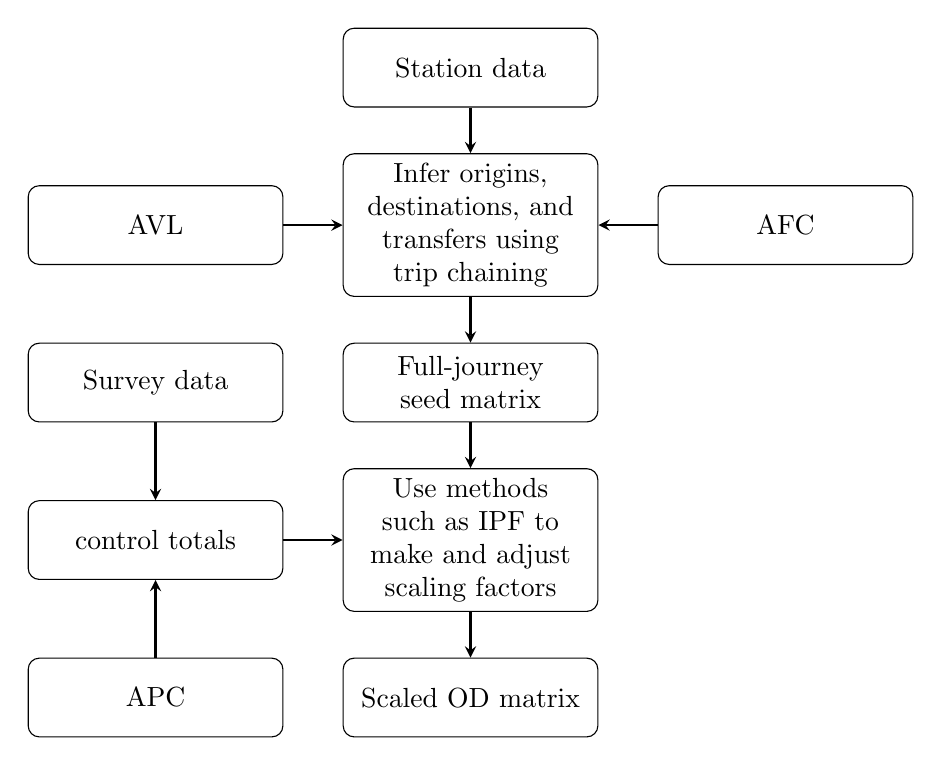
\begin{tikzpicture}[node distance=2cm]

%\node (start) [startstop] {Read (Station data, Schedule data, AFC, AVL)};
\node (start) [startstop]  {Infer origins, destinations, and transfers using trip chaining};

\node (io1) [startstop, right of=start, xshift=2cm] {AFC};
\node (io2) [startstop, left of=start, xshift=-2cm] {AVL};
\node (io3) [startstop, above of=start] {Station data};


\node (pro2) [startstop, below of=start]  {Full-journey seed matrix};
\node (pro3) [startstop, below of=pro2]  {Use methods such as IPF to make and adjust scaling factors};
\node (pro4) [startstop, below of=pro3]  {Scaled OD matrix};



%\node (pro5) [startstop, right of=pro3, xshift=2cm]  {Scale the matrix};
\node (pro6) [startstop, left of=pro3, xshift=-2cm]  {control totals};

\node (io4) [startstop, above of= pro6] {Survey data};
\node (io5) [startstop, below of=pro6] {APC};


\draw [arrow] (io1) -- (start);
\draw [arrow] (io2) -- (start);
\draw [arrow] (io3) -- (start);

\draw [arrow] (io4) -- (pro6);
\draw [arrow] (io5) -- (pro6);

\draw [arrow] (start) -- (pro2);
\draw [arrow] (pro2) -- (pro3);
\draw [arrow] (pro3) -- (pro4);
%\draw [arrow] (pro5) -- (pro3);
\draw [arrow] (pro6) -- (pro3);

\end{tikzpicture}

\caption{Flow chart of general OD matrix estimation approach.}
\end{center}
\end{figure}





\newpage
\section{Summary of key methods for origin-destination inference in transit systems}
%Here, you want to summarize and give an overview of the basic ODX estimation approaches.
%You could use a table or figure, etc...

%The IPF (iterative proportional fitting or biproportional fitting), minimum cost path, and Route level ODX with AFC and AVL are Some of the methods used for ODX  

ADCS have become increasingly available in recent years, and with the different characteristics and types data available to different transit agencies, different methodologies have been developed.

%O-D matrix estimation models can be broadly divided into traffic modeling based approaches and statistical inference based approaches. The former include the minimum information/ entropy maximizing models and combined models for traffic planning (Van Zuylen and Willumsen, 1980; Bell, 1983; Yang, 1995; Wong et al., 2005), and the latter include the maximum likelihood method and generalized least squares method (Mather, 1983; Cascetta, 1984; Spiess, 1987; Bell, 1991; Lo et al., 1996, 1999; Chan and Lo, 2001). \citep{wongEstimationOrigindestinationMatrices2005}


\subsection{Trip Chaining}
Trip chaining is a process where passengers take at least one connection from one travel vehicle to another \citep{huangMethodBusOD2020}. This method is used to infer alighting stops based on entry-only fare card transaction and AVL data which is an essential step in obtaining a seed matrix.  \citep{cuiBusPassengerOriginDestination2006}. 


Trip Chaining infers passenger trips to by connecting trip legs when the criteria for a transfer between them are met. It creates buffer zones around each boarding location to infer the alighting location that preceded it. These buffer zones are based on the following general assumptions\citep{alsgerValidatingImprovingPublic2016}:
\begin{itemize}

\item Allowable transfer time

This value ranges from 30 min to 90 min in previous research \citep{alsgerValidatingImprovingPublic2016}.


\item Allowable walking distance

Similarly, different walking distances were used ranging from 400 m to 1100 m \citep{alsgerValidatingImprovingPublic2016}.


\item Last destination 

The most common of the two assumptions used for the last destination is that the last alighting location of the day is the same as the fist boarding location of that day. But the more realistic assumption is to choose the closest stop on the last trip's route to the first boarding location as the last destination \citep{alsgerValidatingImprovingPublic2016}.





% for rail systems according to {cuiBusPassengerOriginDestination2006}. 

%\item Passengers' next trip starts at the destination station of their previous trip  (next trip method) or at another station colse by. \citep{cuiBusPassengerOriginDestination2006}. 

%\item Passengers last trip of the day ends at the first origin station of that day (last trip of the day method) \citep{cuiBusPassengerOriginDestination2006}. 

%\item If a bus is used, the intersection between the bus and rail routes indicates the alighting location \citep{zhaoPlanningAnalysisImplications2004}.


\end{itemize}


%\subsection{Gravity model}


%\subsection{Logit model}


%\subsection{Minimum path}



\subsection{Minimum Information/ Maximum Entropy}

%ME theory (or minimum information theory) was first used by \citep{willumsenSimplifiedTransportModels1981} and \citep{vanzuylenMostLikelyTrip1980a} for the most-likely-trip-matrix estimation problem, based on traffic counts.
The maximum entropy approach is based on the statistical theory of probability and is equivalent to the gravity models \citep{wilsonStatisticalTheorySpatial1967}. This approach is based on the idea that there are many possible trip distributions and that the most probable estimation of the OD matrix is the one that maximizes the total entropy (randomness) \citep{aliDynamicOriginDestinationEstimation}.

%Entropy maximizing techniques have been used as model building tools in transport, urban and regional planning context, particularly after the work of \citep{wilsonEntropyUrbanRegional2011}. For example, it is now conventional to derive most forms of a gravity model from entropy maximizing considerations.
 
%The great attraction of the entropy maximizing and information minimizing models is their generality, their capacity to make full use of the information contained in the observed flows and their flexibility to utilize other available information \citep{willumsenSimplifiedTransportModels1981}.



\subsection{Iterative Proportional Fitting (IPF)}

IPF, also referred to as  biproportional fitting and RAS algorithm, is a process in which all the rows are factored proportionately to match their row totals, followed by factoring all the columns. The process is repeated until it converges \citep{navickDistanceBasedModelEstimating1994}. it is related to the entropy maximization technique and considered to be a subset of it \citep{lovelaceEvaluatingPerformanceIterative2015}. Its original formulation is attributed to\citep{demingLeastSquaresAdjustment1940}.

IPF is usually used to estimate a single route OD matrix from a seed matrix and the total boarding and alighting counts as control totals.  A modified IPF or a Proportional distribution methods are used to estimate OD matrices on the network level \citep{cuiBusPassengerOriginDestination2006}. 

IPF is more desirable than other matrix expansion methods due to ''its computational ease without loss of accuracy'' \citep{ben-akivaALTERNATIVEMETHODSESTIMATE1985}.


\subsection{Maximum Likelihood Estimation (MLE)}

Similar to IPF, this method is used to estimate a single route OD matrix. But to use MLE, only a sample of Passenger flows and a sample of boarding and alighting counts, instead of totals, are needed \citep{cuiBusPassengerOriginDestination2006}. 


\subsection{Bayesian Approach}
(``Bayesian methods allow us to estimate model parameters, to construct model forecasts and to conduct model comparisons.'' ''In the Bayesian context, a model is defined by a likelihood function and a prior.'' ``Under the maximum likelihood approach, the model parameters are interpreted as fixed and the observed data represents a particular draw from the likelihood function. Parameter estimation then requires the maximization of the likelihood function.'' ``By contrast, the Bayesian approach interprets the parameters as random variables.'' \citep{BayesianMethodOverview}.)<>





%We assume a mathematical representation of the physical system of interest which consists a set of input, output and state variables related by first-order differential equations. State variables take values that evolve over time and depend on the values they have at a given time t and the input variables. The measurements take values which depend on the state variables. \citep{englezouBayesianEstimationOriginDestination2019}


%\subsection{Dynamic models}
%models take for granted	that	transportation	systems are stationary, meaning parameters such as	 mean OD flows and variances do	not vary	over time (static).But in	reality, transportation systems are non-stationary, since social-economic conditions,	infrastructure and other	factors	change over time. Dynamic models were developed to model the dynamic variation of the demand in order to predict future behavior of the system or to assess the impact of interventions in the system over time \citep{netoStatisticalModelsEstimation2017}.



%\subsection{least squares method}


%\subsection{Spatial Clustering}

%In understanding travel behavior (individual/aggregated), clustering techniques such as density-based spatial clustering, K-means clustering, and Gaussian mixture model are generally applied. \citep{zannatEmergingBigData2019}. 
%It is used to group passengers based on their travel patterns \citep{vanderwaartPlanningTransitNetworks2016}.


%Table 1 summarizes some articles that used these methods and their case studies

\begin{longtable}[c]{l|l|l} 
  \caption{Summary of Articles that used the above OD estimation methods}
  \label{tab:table1}\\
  \toprule
  \textbf{Method} & \textbf{Article} & \textbf{Case Study}\\

  \midrule
  \endfirsthead 
  \toprule
  \textbf{Method} & \textbf{Article} & \textbf{Case Study}\\

  \midrule
  \endhead 


      \multirow{4}{*}{Bayesian Approach}  &  \citep{zhuAgentBasedRouteChoice2018} & The Flanders Belgian region\\
      & \citep{hazeltonStatisticalInferenceTransit2010} & Bus service in San Francisco Bay\\
      & \citep{liBayesianInferenceOriginDestination2005} & RA region, Leicester \\
      &  \citep{perrakisBayesianApproachModeling2012}& The Flanders region, Belgium\\
      
      
      
      \midrule

      \multirow{4}{*}{IPF}  & \citep{cuiBusPassengerOriginDestination2006} & Chicago Transit Authority (CTA) bus network\\
      & \citep{zhaoEstimatingRailPassenger2007} & Chicago Transit Authority (CTA) rail system\\
      & \citep{navickDistanceBasedModelEstimating1994} &  The Boston area\\
      & \citep{gordonIntermodalPassengerFlows2012}&  London public transit system\\
      
      
      
      \midrule

      \multirow{2}{*}{MLE}  &  \citep{cuiBusPassengerOriginDestination2006} & Chicago Transit Authority (CTA) bus network\\
      & \citep{navickDistanceBasedModelEstimating1994} & The Boston area\\

%removed Gravity model and put it with MI and ME

      \midrule

      \multirow{5}{*}{MI/ME/GM}  & \citep{wongEstimationOrigindestinationMatrices2005} & Hong Kong multimodal transit network\\
%find a way to put the full names (minimum info, maximum entropy, gravity model)
      & \citep{geUpdatingOriginDestination2016} & Tokyo City\\
      & \citep{tongSchedulebasedDynamicTransit2001} & The MTR system in Hong Kong\\
      & \citep{wongESTIMATIONMULTICLASSORIGINDESTINATION2005} & Hong Kong highway network\\
      & \citep{ekowicaksonoEstimatingOriginDestinationMatrix2016} & Bogor City\\

      \midrule


      \multirow{4}{*}{Trip Chaining}  & \citep{widyawanBigDataAnalytic2017} & Public transport of Jakarta, Indonesia\\
      & \citep{zhaoEstimatingRailPassenger2007} & Chicago Transit Authority (CTA) rail system\\
      & \citep{huangMethodBusOD2020}& Suzhou,China\\
      & \citep{nassirTransitStopLevelOrigin2011} & Minneapolis–Saint Paul, Minnesota\\
      & \citep{wangBusPassengerOrigindestination2010} & London TFL network\\






%      \midrule

%      Spatial Clustering & \citep{luoConstructingTransitOrigin2017} & Haaglanden, Netherlands\\


  \bottomrule
\end{longtable}





\section{Impact on Sustainability}
Public transit is considered an important tool for sustainability \citep{miller2016analyzing}. Therefore, when planning transit networks, there is a need to know how to use the available infrastructure more efficiently and what is the most effective investment to make given the available resources \citep{peterson2007origindestination}.

Big data based OD estimation has the potential to be a very efficient and effective approach because it uses real data instead of relying on samples provided by surveys. That helps planners understand the exact details of what modes people are using, how long they take while traveling, and where they are traveling to and from. This makes the decisions made by agencies more accurate and therefore can help in making transportation more sustainable by cutting unnecessary transit schedules and reducing travel time.

This sustainability means the improvement to the quality of life, the reduction of emissions and energy consumption, and has many economic benefits as a result of the increased efficiency \citep{henke2020decisionmaking}.









%\section{Summary of success/impact stories}
%Where have ODX models been applied with success? What have been the benefits especially to planning/resilience/disruption? Geographical considerations, etc..

\section{The PVTA System}
%Also here, there can be a brief historical component of the PVTA system...

''The Pioneer Valley Transit Authority (PVTA) was created in 1974 under M.G.L. Chapter 161B and is the second largest transit agency in Massachusetts. PVTA provides public transportation services to 24 communities in Hampden and Hampshire Counties, and serves 21 Opportunity Zones. PVTA's service area covers over 600 sq. mi. and a population of almost 600,000. In FY19, PVTA provided over 10 Million fixed route rides and over 250,000 paratransit trips. PVTA’s fixed route system is split into three main areas: Springfield Area Transit Company (SATCo), which operates in the southern portion of Hampden County and typically serves 60 percent of riders, UMass Transit Services (UMTS/UMass), which operates PVTA's routes in the Five College area in eastern Hampshire County and serves 31 percent of riders on average, and Valley Area Transit Company (VATCo), which operates in the northwest portion of PVTA's service area and serves approximately 9percent of riders.''


''The Pioneer Valley Transit Authority (PVTA) was created in 1974 under M.G.L. Chapter 161B and is the second largest transit agency in Massachusetts. PVTA provides public transportation services to 24 communities in Hampden and Hampshire Counties, and serves 21 Opportunity Zones. PVTA's service area covers over 600 sq. mi. and a population of almost 600,000. In FY19, PVTA provided over 10 Million fixed route rides and over 250,000 paratransit trips. PVTA’s fixed route system is split into three main areas: Springfield Area Transit Company (SATCo), which operates in the southern portion of Hampden County and typically serves 60 percent of riders, UMass Transit Services (UMTS/UMass), which operates PVTA's routes in the Five College area in eastern Hampshire County and serves 31 percent of riders on average, and Valley Area Transit Company (VATCo), which operates in the northwest portion of PVTA's service area and serves approximately 9percent of riders.''

\begin{itemize}
\item A Brief History 


\item Motivation

%\item Other transit services

\end{itemize}




%\section{Conclusion}
%\begin{itemize}


%{
%\item Gaps in research
%Existing algorithms and models in the con-temporary studies to predict origin, destination, and route choice have many applications and substantial level of accuracy. But, the develop-ment of these models involved multiple steps and considered many assumptions and sampling approximation. While the validity of these mod-els depends on the accuracy of these assumptions and sampling approximation, very few attempts have been made to validate these assumptions in a context different from the training/estimation context53. Therefore, future research is needed to propose new techniques to validate the underly-ing assumptions in PT modeling using big data and potentially provide insights about their fore-casting performance. \citep{zannatEmergingBigData2019}

%Further, though there are possibilities of com-bining multiple big data sources or big and small data for PT planning (e.g., smart card data with mobile phone data), only few studies have focused on this aspect on a limited scale. There is poten-tiality to develop wide-scale models combin-ing land use, weather, events, and other big data sources to understand travel behavior in differ-ent landscapes. While there exist various sources of big data, methods to integrate these different types of data to solve problems (e.g., congestion and service deficiency), which could improve the accuracy in predicting individual travel behavior, do not exist. \citep{zannatEmergingBigData2019}Existing sources of big data are often criticized for not providing information such as socio-demographic characteristics of the passen-gers. Integrating data collected from small-scale surveys and correcting the potential biases with the big data sources (as proposed by Bwambale et al.15 in the context of generic travel behavior) can provide more insights into travel behavior. \citep{zannatEmergingBigData2019}

%In addition, cross-cutting research is needed to explain the applicability of big data in the extended domain of PT, such as spatio-temporal relation-ship between origin and destination choice, transit users’ transfer choice, and mode choice behavior19. Besides, disjointed O–D estimation, route choice, transfer choice, and mode choice research can be integrated to understand the complex trip chain and travel behavior25. Trip-chaining and linked trip analysis can be further extended for infer-ring trip purpose, analyzing spatial and temporal travel pattern, and analyzing route choice behavior of passenger32, 39. To improve the performance of PT service, research is needed to determine the relationship between passenger travel demand and performance indicator such as speed of vehicle, quality of service, accessibility to PT, and passenger waiting time22, 43, 64. \citep{zannatEmergingBigData2019}

%In understanding travel behavior (individual/aggregated), clustering techniques such as den-sity-based spatial clustering, K-means++ cluster-ing, and Gaussian mixture model are generally applied. However, application of supervised clas-sification process, interpretation, and validation with onboard data are needed to classify the het-erogeneous transit user42. But, to understand activity-based travel behavior in PT use, none of the studies have either used big data in develop-ing agent-based individual model or imple-mented model in an open-sourced agent-based micro-simulation tool5. Therefore, advanced mathematical model, machine learning toolkit, and application of spatial statistics integrated with spatial analysis are needed to understand the interaction of PT user with the surroundings. Since, big data has the potentiality to provide both short-/long-term records, future research can evaluate alternative scenarios of different PT policy environment (e.g., before and after policy implementation), which will enable to under-stand the potential impacts of a PT policy4, 22.\citep{zannatEmergingBigData2019}

%Finally, apart from a few reviewed papers, big data has been used in transport research predom-inantly in context of developed countries, similar uses of such data in planning and operation of PT system is needed in developing countries, where the PT landscape is changing morerapidly. It is expected that in future the accuracy and precision of the PT data will improve over time leading to fewer missing data and gaps in the trajectory. The improved data quality holds the promise of leading to more robust PT planning models. A more promising direction is, however, the emergence of multimodal data (e.g., data from ride-sharing modes, shared bikes). These emerging data sources are promising for PT plan-ning from two aspects. Firstly, such data can be leveraged to optimize the transport network as a whole as opposed to PT only. Secondly, they can be used to infer the latent PT demand and take PT planning measures to maximize the revenue. \citep{zannatEmergingBigData2019}

%This review could be a useful guide for fellow researchers who intend to work with “big data” and “PT planning”, which will contribute in promoting PT. Despite the ever-increasing demand for car use, hopefully, academic research with big data will provide useful guideline on how to reduce car use considering the current situation of PT usage. Hence, exploring new methods and techniques is essential to employ big data in accu-rately explaining travel behavior and improving PT system. \citep{zannatEmergingBigData2019}


%}



%\item What is currently missing? Where is there room for improvement? What are the potential benefits yet to be realized

%\end{itemize}
%Frame these questions within the context of the PVTA?   

\printbibliography

\end{document}

%%% Local Variables:
%%% mode: latex
%%% TeX-master: t
%%% End:
